\section[Intuition and Definitions]{Intuition and Definitions}

\subsection[Intuition]{Intuition}

\begin{frame}{Case Study Presentation}
	We will consider the following case study:
	\begin{itemize}
		\item Suppose we want to determine the average height of individuals on the University of Toulouse 3 campus.
		\pause
		\item There exists a \textbf{true} value. This is the value we would obtain if we measured \textit{everyone}.
		\pause
		\item In practice, we will work with \textbf{samples}.
	\end{itemize}
\end{frame}

\begin{frame}{Interval Construction}
	For the prediction interval:
	\begin{itemize}
		\item We collect the heights of $n$ students.
		\item We seek a maximum likelihood estimator for the \textbf{heights} using a Gaussian distribution.
		\item We calculate the centered interval representing 95\% of the measured \textbf{heights}.
	\end{itemize}
	\pause
	For the confidence interval:
	\begin{itemize}
		\item We generate $m$ samples:
		\begin{itemize}
			\item We collect the heights of $n$ students.
			\item We calculate the sample mean height.
		\end{itemize}		
		\item We seek a maximum likelihood estimator for the \textbf{means} using a Gaussian distribution.
		\item We calculate the centered interval representing 95\% of the measured \textbf{means}.
	\end{itemize}
\end{frame}

\begin{frame}{Results with $n = 30$ and $m = 100$}
	\begin{columns}
		\begin{column}{0.5\textwidth}
			\begin{figure}
				\centering
				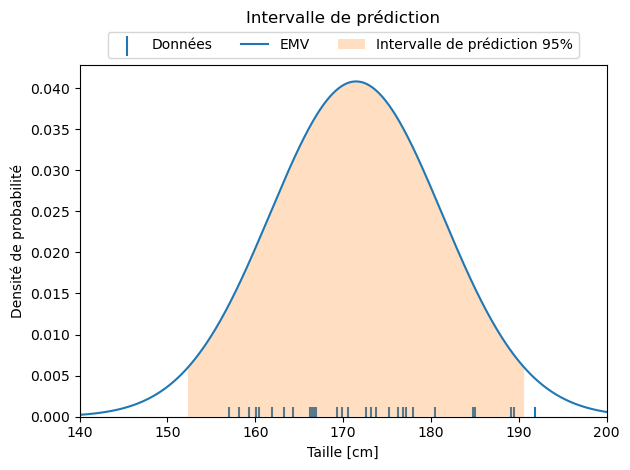
\includegraphics[width=1.0\linewidth]{Images/intervalle_prediction_n30}
				\label{fig:prediction-interval-n30}
			\end{figure}
		\end{column}
		\begin{column}{0.5\textwidth}
			\begin{figure}
				\centering
				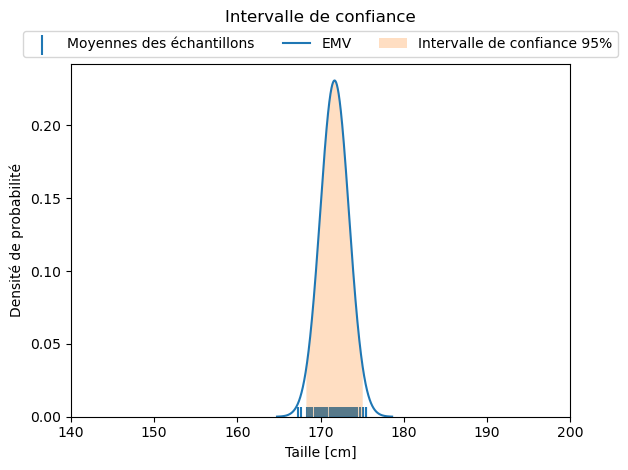
\includegraphics[width=1.0\linewidth]{Images/intervalle_confiance_n30}
				\label{fig:confidence-interval-n30}
			\end{figure}
		\end{column}
	\end{columns}
\end{frame}

\begin{frame}{Results with $n = 300$ and $m = 100$}
	\begin{columns}
		\begin{column}{0.5\textwidth}
			\begin{figure}
				\centering
				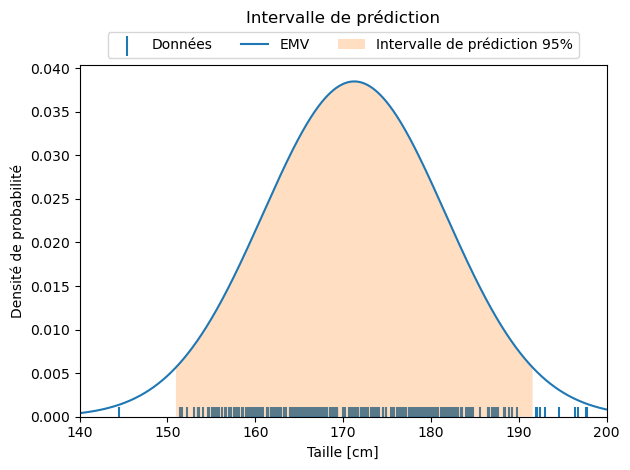
\includegraphics[width=1.0\linewidth]{Images/intervalle_prediction_n300}
				\label{fig:prediction-interval-n300}
			\end{figure}
		\end{column}
		\begin{column}{0.5\textwidth}
			\begin{figure}
				\centering
				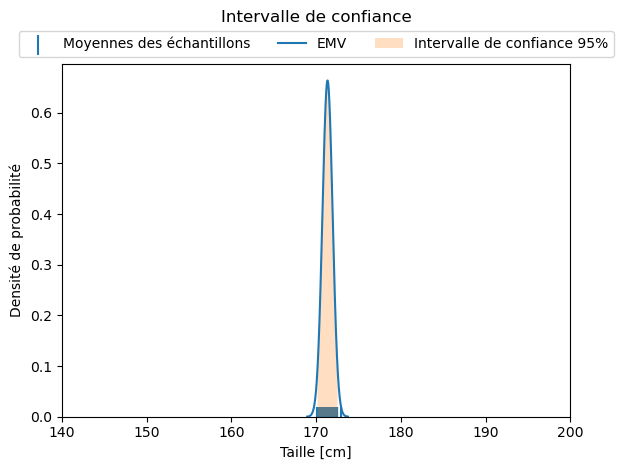
\includegraphics[width=1.0\linewidth]{Images/intervalle_confiance_n300}
				\label{fig:confidence-interval-n300}
			\end{figure}
		\end{column}
	\end{columns}
\end{frame}

\begin{frame}{Discussion}
	\begin{itemize}
		\item The prediction interval changes only very slightly as the sample size increases.
		\item The confidence interval narrows as the sample size increases.
		\item The prediction interval measures the height disparity within a sample.
		\item The confidence interval measures the disparity of the mean across multiple samples.
	\end{itemize}
	\pause
	\vspace{0.5cm}
	The standard deviation of the confidence interval, called the \textbf{standard error} ($\ET$), decreases as the sample size increases. It varies as $1 / \sqrt{n}$.
\end{frame}

\begin{frame}{Interpretation}
	\begin{itemize}
		\item A 95\% prediction interval means that 95\% of future observations will fall within this interval.
		\pause
		\item A 95\% confidence interval means that 95\% of future sample means, calculated in an identical manner, will fall within this interval.
		\pause
		\item Note that the 95\% coverage is not \textbf{guaranteed}. It depends on the validity of the assumptions, particularly the Gaussian nature of the distributions.
	\end{itemize}
	\pause
	If the standard deviation of the height of a group of students $\sigma$ is known, the standard error $\ET$ can be calculated from the sample size $n$:
	\begin{equation}
		\ET = \frac{\sigma}{\sqrt{n}}
		\nonumber
	\end{equation}
\end{frame}